%%%%%%%%%%%%%%%%%%%%%%%%%%%%%%%%%%%%%%%%%%%%%%%%%%%%%%%%%%%%%%%%%%%%%%
% This layout was adapted from one found at latextemplates.com which
% was adapted from another.
%
% License: CC BY-NC-SA 3.0
% (http://creativecommons.org/licenses/by-nc-sa/3.0/)
%
% Original header:
%
% This is a LaTeX version of the sample laboratory report from
% Virginia Tech's copyrighted 08-09 CHEM 1045/1046 lab manual.
% Reproduction of this one appendix section for academic purposes
% should fall under fair use.
%
%%%%%%%%%%%%%%%%%%%%%%%%%%%%%%%%%%%%%%%%%%%%%%%%%%%%%%%%%%%%%%%%%%%%%%

\documentclass{article}

\usepackage{graphicx}
%\usepackage[acronym]{glossaries} % Lets us use acronyms
\usepackage{multicol}
\usepackage{amsmath}
\usepackage{siunitx} % SI units in math mode
\usepackage{subcaption}

\author{}
\title{ELEC-313 \\ Lab 3: Diode Circuits\\ }
\date{\today}

%\loadglsentries{acronyms} % Actually loads 'acronyms.tex'
%\makeglossaries

\begin{document}

\maketitle

\begin{center}
  \begin{tabular}{lr}
    Date Performed: & September 25, 2013 \\
    Partners: & Charles Pittman \\
    & Stephen Wilson \\
  \end{tabular}
\end{center}

\newpage

\tableofcontents
\listoffigures
\listoftables

\newpage

% Number the enumerate environment (unordered lists) by letter:
\renewcommand{\labelenumi}{\alph{enumi}.}

\section{Objective}
\label{sec:objective}

The objective is to construct, measure, and observe the behavior of two common diode circuits: a voltage rectifier, and a voltage regulator.

\section{Equipment}
\label{sec:equipment}

\begin{tabular}{ll}
  \centering
  Diode: 1N4007 & Power supply: HP E3631A \\
  Zener diode: 1N5231 & Function generator: HP 33120A \\
  Resistors: \SI{47}{\ohm} & Multimeter: Fluke 8010A \\
  Capacitor: \SI{1}{\micro\farad} & Oscilloscope: Agilent 54622D \\
  Resistive decade box: HeathKit IN-3117 \\
\end{tabular}

\section{Schematics}
\label{sec:schematics}

\begin{figure}[hbtp]
  \centering
  \begin{subfigure}[b]{0.6\textwidth}
    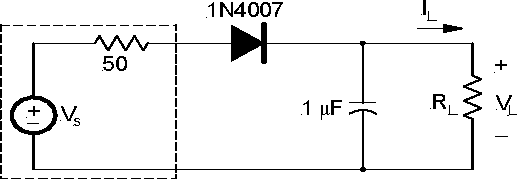
\includegraphics[width=\textwidth]{volt_rect}
    \caption{\label{fig:volt_rect} Voltage rectifier circuit.}
  \end{subfigure}%
  ~
  \begin{subfigure}[b]{0.4\textwidth}
    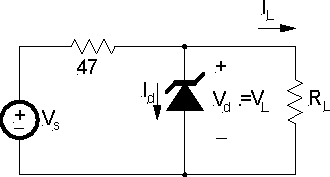
\includegraphics[width=\textwidth]{volt_reg}
    \caption{\label{fig:volt_reg} Voltage regulator circuit.}
  \end{subfigure}
  \caption{\label{fig:circuits_tested} Circuits used in this lab.}
\end{figure}

\section{Procedure}
\label{sec:procedure}

\subsection{Voltage Rectifier}
\label{sec:rectifier}

First, the capacitance of a \SI{1}{\micro\farad} capacitor was measured and  recorded in Table~\ref{tab:cap} along with the percent difference calculated (Eq~\label{eq:percent_diff}).  Then the circuit shown in Figure~\ref{fig:volt_rect} was constructed on a breadboard. The voltage source ($V_S$) and \SI{50}{\ohm} resistor seen in Figure~\ref{fig:volt_rect} represented the function generator used.  Using a resistive decade box, the load resistance ($R_L$) was initially set to \SI{10}{\kilo\ohm}.  Then, the first channel of the oscilloscope was set to measure the output of the function generator and the second channel was set to measure the voltage across the load ($V_L$).  The function generator was programmed to produce a sine wave of \SI{1}{V_{peak}} at \SI{400}{\hertz}, measured with the oscilloscope.  $V_{max}$, $V_{min}$, and DC voltage across $V_L$ was measured with a multimeter and recorded in Table~\ref{tab:rect_vp_vdc} along with the ripple voltage $V_r$ (Eq~\ref{eq:ripple}).  Finally, the source voltage was then left at \SI{5}{V_{peak}}, and $R_L$ was adjusted to \SI{1}{\kilo\ohm} and \SI{100}{\kilo\ohm} and each $V_{DC}$, $V_{max}$, $V_{min}$, and $V_r$ were measured and recorded in Table~\ref{tab:load_v_ripple}.

\subsection{Voltage Regulator}
\label{sec:volt_reg}

First, a \SI{47}{\ohm} resistor was measured and its \% difference from the nominal resistance value was calculated and both values were recorded in Table~\ref{tab:res}. The circuit shown in Figure~\ref{fig:volt_reg} was constructed on a breadboard, the HP power supply for the voltage source ($V_S$) set to 9 V, and a decade resistance box as the load resistance ($R_L$) set to \SI{1}{\kilo\ohm}. Then the load voltage ($V_L$) and load current ($I_L$) was measured and recorded in Table~\ref{tab:volt_reg_meas}, for the $R_L$ of \SI{1}{\kilo\ohm}, \SI{330}{\ohm}, and \SI{100}{\ohm}. The Zener diode was removed and the open-circuit voltage ($V_{OC}$) was measured and recorded in Table~\ref{tab:volt_reg_meas}, again for the $R_L$ of \SI{1}{\kilo\ohm}, \SI{330}{\ohm}, and \SI{100}{\ohm}. The Zener diode was added back into the circuit and, using the $R_L$ of \SI{1}{\kilo\ohm}, \SI{330}{\ohm}, and \SI{100}{\ohm}, the point at which the source drops out of regulation ($V_S$ drop) was determined and recorded in Table~\ref{tab:volt_reg_meas} by sweeping the $V_S$. Finally, the $R_L$ was removed ($R_L$=$\infty$), $V_S$ was set to 9 V, and the voltage across the Zener diode (also $V_L$) was measured and recorded in Table~\ref{tab:volt_reg_meas}.

\section{Results}
\label{sec:results}

\begin{table}[hbtp]
  \centering
  \begin{tabular}{ccc}
    Nominal & Measured & Difference \\
    (\si{\micro\farad}) & (\si{\micro\farad}) & \\
    \hline
    1 & 0.938 & 6.2\% \\
  \end{tabular}
  \caption{\label{tab:cap} Percent difference of capacitor in rectifier circuit.}
\end{table}

\begin{table}[hbtp]
  \centering
  \begin{tabular}{cccccc}
    $V_S$ & $V_{max}$ & $V_{min}$ & $V_r$ & $V_{DC}$ & Ripple \\
    (\si{V_{peak}}) & (\si{V}) & (\si{V}) & (\si{V}) & (\si{V}) & \\
    \hline
    1 & 0.488 & 0.369 & 0.119 & 0.429 & 24.4\% \\
    2 & 1.41 & 1.10 & 0.310 & 1.26 & 22.0\% \\
    3 & 2.39 & 1.88 & 0.510 & 2.14 & 21.3\% \\
    4 & 3.31 & 2.38 & 0.930 & 2.85 & 28.1\% \\
    5 & 4.25 & 3.19 & 1.06 & 3.72 & 24.9\% \\
  \end{tabular}
  \caption{\label{tab:rect_vp_vdc} AC input vs. DC output of rectifier circuit, where $R_L=\SI{10}{\kilo\ohm}$.}
\end{table}

\begin{table}[hbtp]
  \centering
  \begin{tabular}{cccccc}
    $R_L$ & $V_{max}$ & $V_{min}$ & $V_r$ & $V_{DC}$ & Ripple \\
    (\si{\ohm}) & (\si{V}) & (\si{V}) & (\si{V}) & (\si{V}) & \\
    \hline
    1k & 4.13 & 0.440 & 3.69 & 2.29 & 89.3\% \\
    10k & 4.25 & 3.19 & 1.06 & 3.72 & 24.9\% \\
    100k & 4.321 & 4.193 & 0.128 & 4.257 & 2.962\% \\
  \end{tabular}
  \caption{\label{tab:load_v_ripple} Effect of $R_L$ on DC output in rectifier circuit.}
\end{table}

\begin{figure}[hbtp]
  \centering
  % GNUPLOT: LaTeX picture
\setlength{\unitlength}{0.240900pt}
\ifx\plotpoint\undefined\newsavebox{\plotpoint}\fi
\sbox{\plotpoint}{\rule[-0.200pt]{0.400pt}{0.400pt}}%
\begin{picture}(1500,900)(0,0)
\sbox{\plotpoint}{\rule[-0.200pt]{0.400pt}{0.400pt}}%
\put(171.0,131.0){\rule[-0.200pt]{4.818pt}{0.400pt}}
\put(151,131){\makebox(0,0)[r]{ 0}}
\put(1419.0,131.0){\rule[-0.200pt]{4.818pt}{0.400pt}}
\put(171.0,212.0){\rule[-0.200pt]{4.818pt}{0.400pt}}
\put(151,212){\makebox(0,0)[r]{ 0.5}}
\put(1419.0,212.0){\rule[-0.200pt]{4.818pt}{0.400pt}}
\put(171.0,292.0){\rule[-0.200pt]{4.818pt}{0.400pt}}
\put(151,292){\makebox(0,0)[r]{ 1}}
\put(1419.0,292.0){\rule[-0.200pt]{4.818pt}{0.400pt}}
\put(171.0,373.0){\rule[-0.200pt]{4.818pt}{0.400pt}}
\put(151,373){\makebox(0,0)[r]{ 1.5}}
\put(1419.0,373.0){\rule[-0.200pt]{4.818pt}{0.400pt}}
\put(171.0,454.0){\rule[-0.200pt]{4.818pt}{0.400pt}}
\put(151,454){\makebox(0,0)[r]{ 2}}
\put(1419.0,454.0){\rule[-0.200pt]{4.818pt}{0.400pt}}
\put(171.0,534.0){\rule[-0.200pt]{4.818pt}{0.400pt}}
\put(151,534){\makebox(0,0)[r]{ 2.5}}
\put(1419.0,534.0){\rule[-0.200pt]{4.818pt}{0.400pt}}
\put(171.0,615.0){\rule[-0.200pt]{4.818pt}{0.400pt}}
\put(151,615){\makebox(0,0)[r]{ 3}}
\put(1419.0,615.0){\rule[-0.200pt]{4.818pt}{0.400pt}}
\put(171.0,695.0){\rule[-0.200pt]{4.818pt}{0.400pt}}
\put(151,695){\makebox(0,0)[r]{ 3.5}}
\put(1419.0,695.0){\rule[-0.200pt]{4.818pt}{0.400pt}}
\put(171.0,776.0){\rule[-0.200pt]{4.818pt}{0.400pt}}
\put(151,776){\makebox(0,0)[r]{ 4}}
\put(1419.0,776.0){\rule[-0.200pt]{4.818pt}{0.400pt}}
\put(171.0,131.0){\rule[-0.200pt]{0.400pt}{4.818pt}}
\put(171,90){\makebox(0,0){ 1}}
\put(171.0,756.0){\rule[-0.200pt]{0.400pt}{4.818pt}}
\put(330.0,131.0){\rule[-0.200pt]{0.400pt}{4.818pt}}
\put(330,90){\makebox(0,0){ 1.5}}
\put(330.0,756.0){\rule[-0.200pt]{0.400pt}{4.818pt}}
\put(488.0,131.0){\rule[-0.200pt]{0.400pt}{4.818pt}}
\put(488,90){\makebox(0,0){ 2}}
\put(488.0,756.0){\rule[-0.200pt]{0.400pt}{4.818pt}}
\put(647.0,131.0){\rule[-0.200pt]{0.400pt}{4.818pt}}
\put(647,90){\makebox(0,0){ 2.5}}
\put(647.0,756.0){\rule[-0.200pt]{0.400pt}{4.818pt}}
\put(805.0,131.0){\rule[-0.200pt]{0.400pt}{4.818pt}}
\put(805,90){\makebox(0,0){ 3}}
\put(805.0,756.0){\rule[-0.200pt]{0.400pt}{4.818pt}}
\put(964.0,131.0){\rule[-0.200pt]{0.400pt}{4.818pt}}
\put(964,90){\makebox(0,0){ 3.5}}
\put(964.0,756.0){\rule[-0.200pt]{0.400pt}{4.818pt}}
\put(1122.0,131.0){\rule[-0.200pt]{0.400pt}{4.818pt}}
\put(1122,90){\makebox(0,0){ 4}}
\put(1122.0,756.0){\rule[-0.200pt]{0.400pt}{4.818pt}}
\put(1281.0,131.0){\rule[-0.200pt]{0.400pt}{4.818pt}}
\put(1281,90){\makebox(0,0){ 4.5}}
\put(1281.0,756.0){\rule[-0.200pt]{0.400pt}{4.818pt}}
\put(1439.0,131.0){\rule[-0.200pt]{0.400pt}{4.818pt}}
\put(1439,90){\makebox(0,0){ 5}}
\put(1439.0,756.0){\rule[-0.200pt]{0.400pt}{4.818pt}}
\put(171.0,131.0){\rule[-0.200pt]{0.400pt}{155.380pt}}
\put(171.0,131.0){\rule[-0.200pt]{305.461pt}{0.400pt}}
\put(1439.0,131.0){\rule[-0.200pt]{0.400pt}{155.380pt}}
\put(171.0,776.0){\rule[-0.200pt]{305.461pt}{0.400pt}}
\put(30,453){\makebox(0,0){$V_{DC} (V)}}
\put(805,29){\makebox(0,0){$V_S (V_{peak})$}}
\put(805,838){\makebox(0,0){Peak Voltage vs. DC Voltage in Rectifier Circuit}}
\put(171,200){\usebox{\plotpoint}}
\multiput(171.00,200.58)(1.184,0.499){265}{\rule{1.046pt}{0.120pt}}
\multiput(171.00,199.17)(314.828,134.000){2}{\rule{0.523pt}{0.400pt}}
\multiput(488.00,334.58)(1.117,0.499){281}{\rule{0.993pt}{0.120pt}}
\multiput(488.00,333.17)(314.939,142.000){2}{\rule{0.496pt}{0.400pt}}
\multiput(805.00,476.58)(1.381,0.499){227}{\rule{1.203pt}{0.120pt}}
\multiput(805.00,475.17)(314.504,115.000){2}{\rule{0.601pt}{0.400pt}}
\multiput(1122.00,591.58)(1.133,0.499){277}{\rule{1.006pt}{0.120pt}}
\multiput(1122.00,590.17)(314.913,140.000){2}{\rule{0.503pt}{0.400pt}}
\put(171,200){\makebox(0,0){$+$}}
\put(488,334){\makebox(0,0){$+$}}
\put(805,476){\makebox(0,0){$+$}}
\put(1122,591){\makebox(0,0){$+$}}
\put(1439,731){\makebox(0,0){$+$}}
\put(171.0,131.0){\rule[-0.200pt]{0.400pt}{155.380pt}}
\put(171.0,131.0){\rule[-0.200pt]{305.461pt}{0.400pt}}
\put(1439.0,131.0){\rule[-0.200pt]{0.400pt}{155.380pt}}
\put(171.0,776.0){\rule[-0.200pt]{305.461pt}{0.400pt}}
\end{picture}

  \caption{\label{fig:rect_vp_vdc} AC input vs. DC output of rectifier circuit, where $R_L=\SI{10}{\kilo\ohm}$}
\end{figure}

\begin{table}[hbtp]
  \centering
  \begin{tabular}{ccc}
    Nominal & Measured & Difference \\
    (\si{\ohm}) & (\si{\ohm}) & \\
    \hline
    47 & 46.52 & 1.13\% \\
  \end{tabular}
  \caption{\label{tab:res} Percent difference of resistor in voltage regulator circuit.}
\end{table}

\begin{table}
  \centering
  \begin{tabular}{ccc}
    $R_L$ & $V_{OC}$ & $V_S$ Drop \\
    (\si{\ohm})  & (\si{V}) & (\si{V}) \\
    \hline
    100 & 6.12 & 7.5 \\
    330 & 7.88 & 5.8 \\
    1k & 8.90 & 5.3 \\
  \end{tabular}
  \caption{\label{tab:volt_reg_calc} Calculated values for voltage regulator circuit}
\end{table}

\begin{table}
  \centering
  \begin{tabular}{cccccc}
    $R_L$ & $V_L$ & $I_L$ & $V_{OC}$ & $V_S$ Drop & Voltage \\
    (\si{\ohm}) & (\si{V}) & (\si{mA}) & (\si{V}) & (\si{V}) & Regulation \\
    \hline
    100 & 5.163 & 50.9 & 6.10 & 7.5 & 5.02\%  \\
    330 & 5.318 & 15.62 & 7.87 & 5.9 & 4.03\% \\
    1k & 5.11 & 5.27 & 8.60 & 5.3 & 1.15\% \\
    $\infty$ & 5.38 & --- & --- & --- & ---\\
  \end{tabular}
  \caption{\label{tab:volt_reg_meas} Measured values for voltage regulator circuit}
\end{table}

\begin{table}
  \centering
  \begin{tabular}{ccccc}
    $R_L$ & $V_{OC}$ & $V_S$ Drop \\
    (\si{\ohm}) & (\% diff) & (\% diff) \\
    \hline
    100 & 0.359\% & 0.0\% \\
    330 & 0.102\% & 1.7\% \\
    1k & 3.327\% & 0.0\% \\
  \end{tabular}
  \caption{\label{tab:volt_reg_diff} Comparison of values for voltage regulator circuit}
\end{table}

\section{Comparison of Results}
\label{sec:comp_of_res}

The PSpice computed values of $V_{OC}$ shown in Table~\ref{tab:volt_reg_calc}, were very close to the measured $V_{OC}$ values (Table~\ref{tab:volt_reg_calc}), and were at most only 3.327\% different (Table~\ref{tab:volt_reg_diff}).  Also, the PSpice computed $V_S$ drop (Table~\ref{tab:volt_reg_calc}) was very close to the measured $V_S$ drop (Table~\ref{tab:volt_reg_meas})and the \% difference was at most only 1.7\% (Table~\ref{tab:volt_reg_diff}) (suggesting that the experimenter may have “peaked” at the computed results and subconsciously (or consciously) noticed the recorded value to be almost exactly the same in all three circumstances).

\section{Conclusion}
\label{sec:conclusion}

As seen in Figure~\ref{fig:rect_vp_vdc}, as the peak voltage of the rectifier circuit increases, the rectifier DC voltage increases.  Also, as load resistance is increased on the rectifier, it decreases the \% ripple as shown in Table~\ref{tab:load_v_ripple}.  This was probably because the increase of resistance reduced the amount of current that could be dissipated from the capacitor over the same amount of time before it was “charged up” again.  Additionally, the \% ripple would likely decrease as the input frequency were increased because there would be a smaller time interval for the capacitor to discharge. 

As shown in Table~\ref{tab:volt_reg_meas}, the voltage regulation (calculated using Equation~\ref{eq:volt_reg}) across the \SI{100}{\ohm} resistor is 5.02\% different than the \SI{5.38}{V} measured when the load resistor was removed from the circuit. This shows that the Zener diode used in the experiment is not an ideal Zener. In the regulator circuit (Figure~\ref{fig:volt_reg}), when $V_S$ is below the Zener diode voltage ($V_Z$), $V_{OC}$ is linearly related to $V_S$. When $V_S$ is above $V_Z$, $V_{OC}$ is almost at a constant value approximately equal to $V_Z$. When $V_S$ is “close” to $V_Z$, the relationship of $V_{OC}$ to $V_S$ is not linearly related and the simplified calculations we learned in class are less effective at computing the $V_{OC}$. 

\section{Equations}
\label{sec:equations}

% LaTeX sees blank lines as a start of another paragraph.  To avoid
% unnecessary vertical spaces between equations, and still visually
% separate in source, put a comment between them.
%
\begin{equation}
  \label{eq:percent_diff}
  \%_{diff} = \frac{|nominal - measured|}{nominal}\times 100\%
\end{equation}
%
\begin{equation}
  \label{eq:ripple}
  V_r = V_{max} - V_{min}
\end{equation}
%
\begin{equation}
  \label{eq:volt_reg}
  \%_{reg} = \frac{V_{load} - V_{no load}}{V_{no load}}\times 100\%
\end{equation}

\end{document}
